Selbstgeführte Schaltungen in Wechselrichter kommen immer häufiger zum Einsatz.\\
In diesem Versuch soll das Funktionsprinzip bei einem einphasigen Wechselrichter praktisch untersucht werden. Insbesondere die typischen Strom- und Spannungsverläufe. Dabei soll untersucht werden wie sich Wirk- und Blindleistung einstellen lassen und welche Auswirkungen dies auf die harmonischen Oberwellen hat.


\subsection{Laboreinrichtung}
\begin{itemize}
\item Mit Netz synchronisierbarer einphasiger Wechselrichter
\item Einphasentransformator, 400V / 230V, 25A
\item Entkopplungsinduktivität 70mH, 30A
\item Maschienensatz zur DC-seitigen Speisung eines Wechselrichters
\end{itemize}

\subsection{Ziele}
\begin{itemize}
\item Überprüfen des theoretisch behandelten Verhalten von selbstgeführten einphasigen Stromrichtern
\item Einstellen der Wirk- bzw. Blindleistung
\item Die Auswirkungen der verschiedenen Pulsmuster auf die harmonischen Oberschwingungen
\end{itemize}

\subsection{Versuchsaufbau}
\begin{figure}[H]
  \begin{center}
  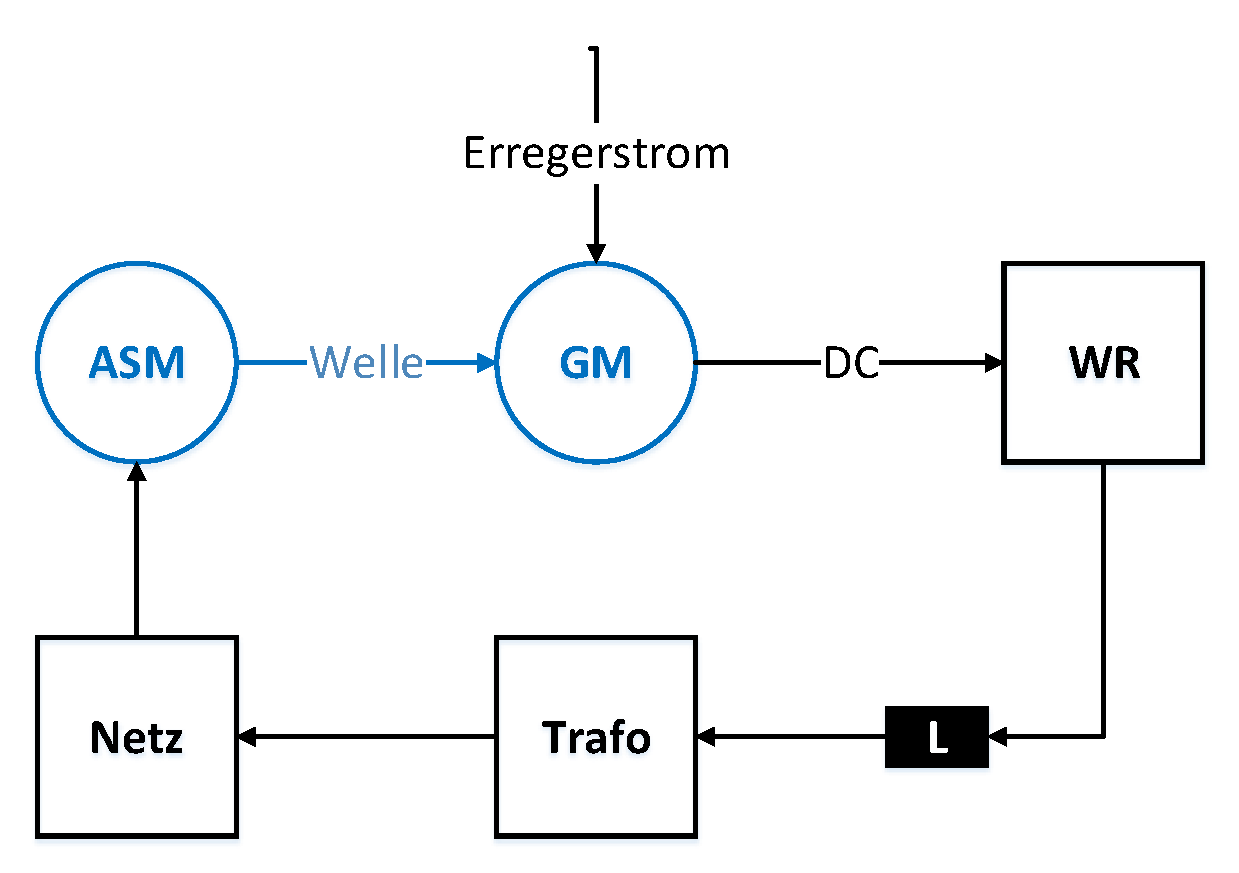
\includegraphics[width=0.5\textwidth]{pic/einleitung/versuchsaufbau.pdf}
  \caption{Versuchsaufbau}
  \label{fig:versuchsaufbau}
  \end{center}
\end{figure}

\clearpage